\section{Analisi di Sensibilità}

L'analisi di sensitività è stata condotta sul modello SEIR, 
come illustrato in Figura \ref{fig:ODE_Julia_example}. 
Questa analisi mirava a valutare come il modello reagisse a 
variazioni specifiche dei suoi parametri, le quali potrebbero 
condurre a comportamenti inattesi o peculiari.

Per effettuare l'analisi di sensitività, sono stati impiegati i 
metodi forniti dalla suite SciML.ai. Ciò ha permesso di identificare 
i parametri ai quali il modello è più sensibile.

\begin{minipage}{\linewidth}
	\centering
	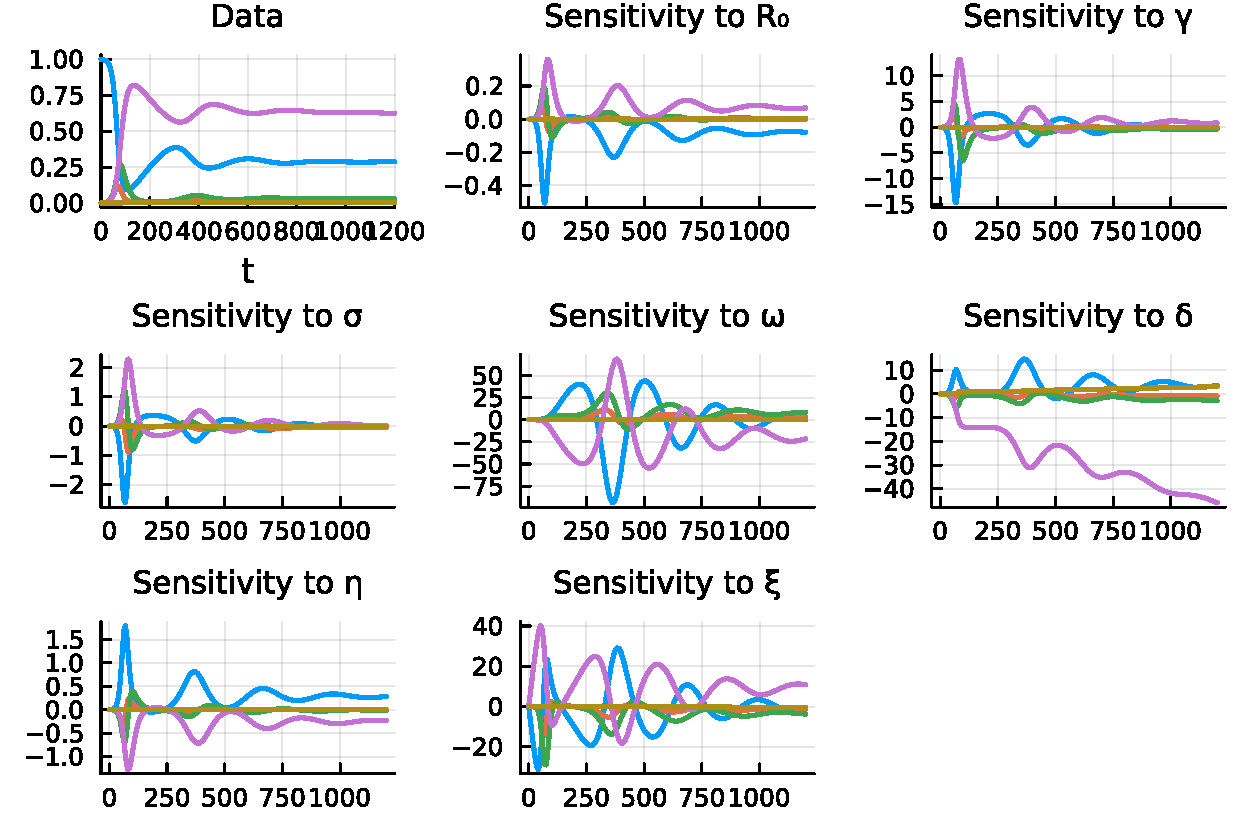
\includegraphics[width=\textwidth]{img/sa.pdf}
	\captionof{figure}{Grafico rappresentante l'analisi di sensitività del modello}
	\label{fig:sens_anal}
\end{minipage}

Come evidenziato nella Figura \ref{fig:sens_anal}, il modello 
dimostra una sensitività uniforme rispetto ai parametri 
$R_0$, $\gamma$, e $\sigma$, il che è coerente, dato che essi 
influiscono sull'andamento dell'epidemia. La sensitività ai parametri 
$\omega$ e $\delta$ era attesa, ma è risultata più marcata di 
quanto previsto. La sensitività al parametro $\eta$, che influisce 
sulle contromisure, è inversamente correlata a quella del 
parametro $R_0$, come previsto, poiché $\eta$ è direttamente 
legato alle misure di contenimento. La sensitività al parametro 
$\xi$ mostra un comportamento singolare, probabilmente dovuto 
alla sua correlazione con $\omega$, entrambi legati al compartimento 
"R" del modello, che gestisce gli individui guariti e vaccinati.

Successivamente, è stata condotta un'analisi di sensitività sui 
parametri specifici del modello ad agenti utilizzando la funzione 
\textbf{paramscan} fornita dalla libreria \textbf{Agents.jl}. 
Sono stati selezionati parametri potenzialmente influenti sul 
comportamento del modello:

\begin{minipage}{\linewidth}
	\centering
	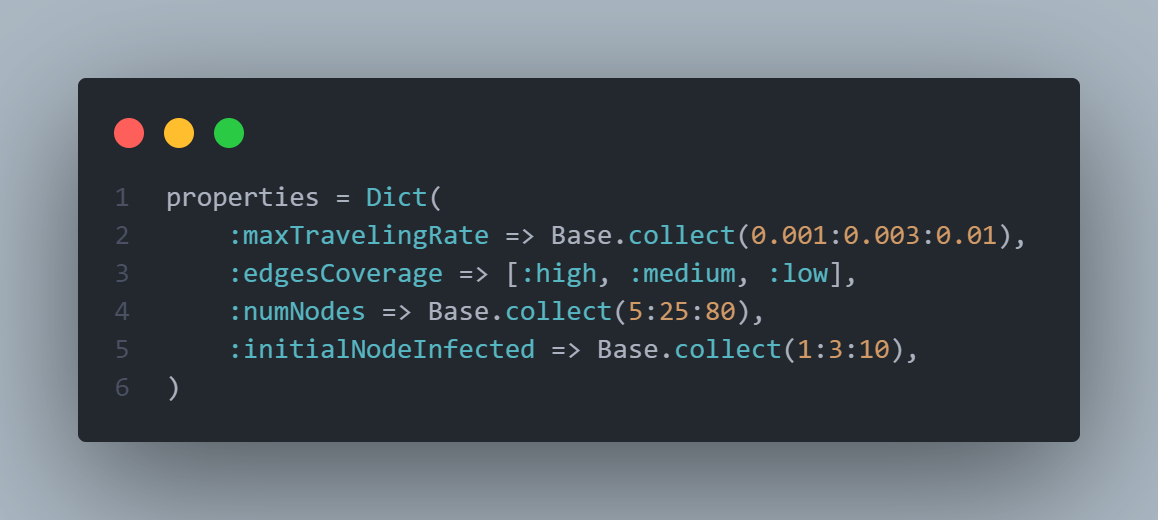
\includegraphics[width=\textwidth]{img/paramscan.png}
	\captionof{figure}{Parametri usati per l'analisi di sensitività del modello ad agente}
	\label{fig:paramscan}
\end{minipage}

Questi parametri sono stati scelti in quanto potenziali 
agenti di cambiamenti significativi nel comportamento del modello. 
I parametri relativi al controllore e al vaccino sono stati esclusi, 
poiché è stato dimostrato che le loro variazioni possono comportare 
cambiamenti significativi nella simulazione.
\newpage

\subsection{Analisi del Comportamento in Base al Numero Iniziale di Nodi Infetti}

L'analisi ha esaminato come il numero iniziale di nodi infetti 
influenzi il comportamento del modello. Si è osservato che un numero 
maggiore di nodi infetti iniziali porta a un raggiungimento più 
rapido del picco di infetti, ma non ha comportato altri comportamenti 
significativi. Questo risultato era atteso e coerente con le 
dinamiche epidemiologiche.

\begin{figure}[!hb]
	\centering
	\begin{subfigure}[b]{0.45\textwidth}
		\centering
		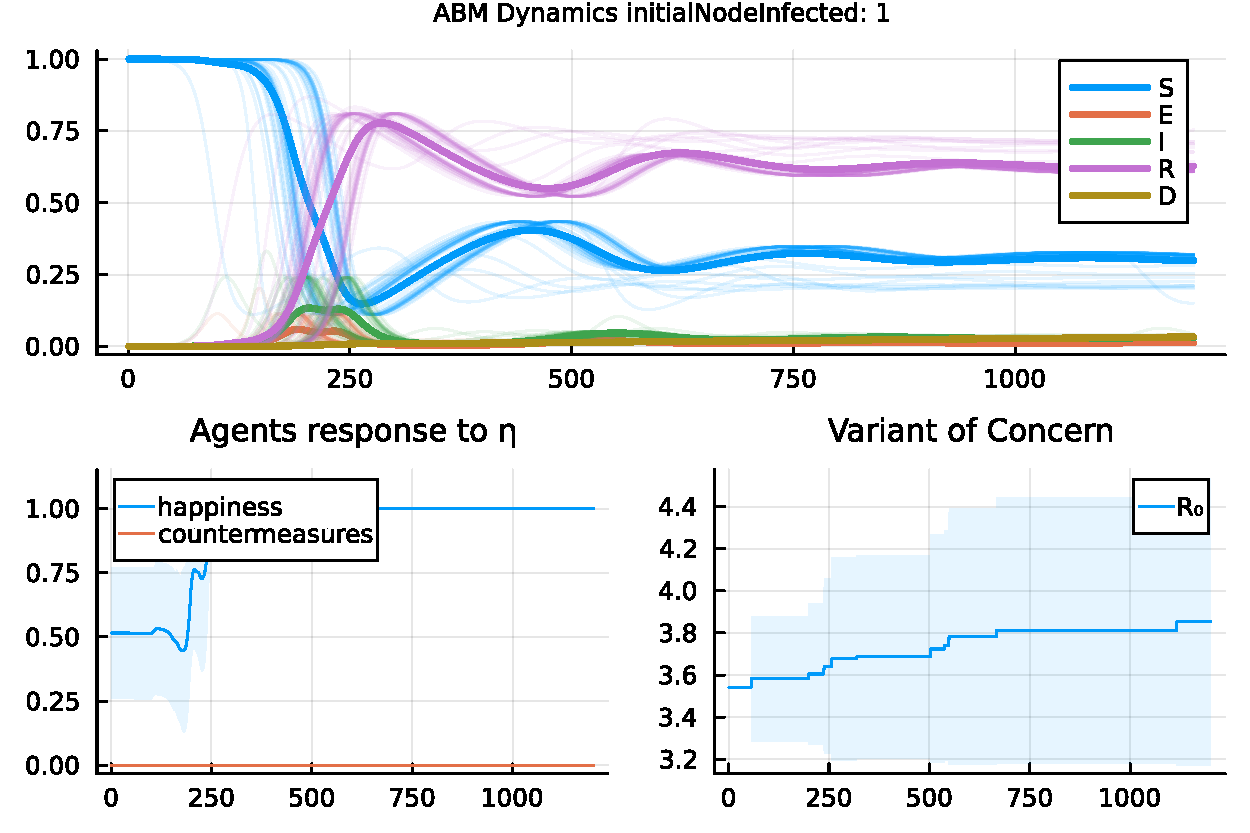
\includegraphics[width=\textwidth]{img/SocialNetworkABM_1_II.pdf}
		\caption{Grafico per la comparazione sul numero di nodi infetti di partenza. Numero nodi infetti iniziali 1}
		\label{fig:comparison_init_node_inf_1}
	\end{subfigure}
	\hfill
	\begin{subfigure}[b]{0.45\textwidth}
		\centering
		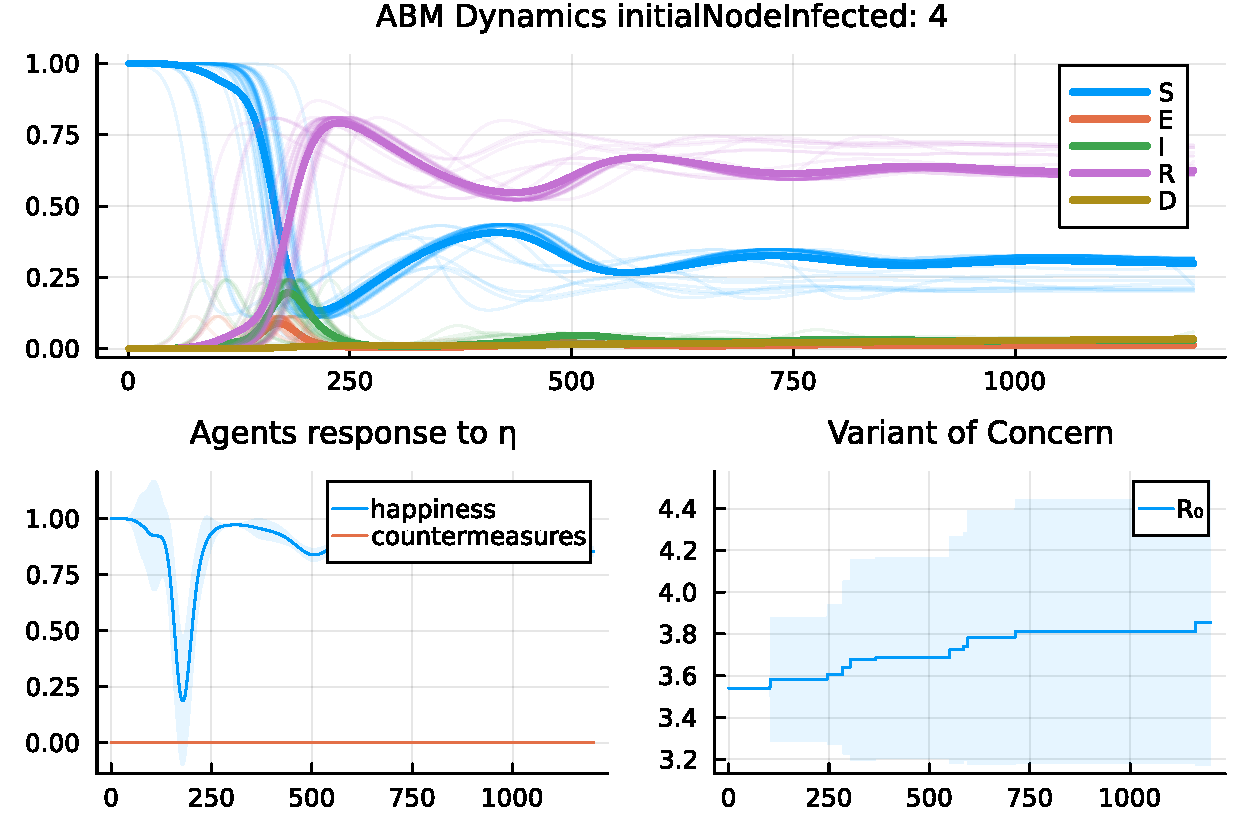
\includegraphics[width=\textwidth]{img/SocialNetworkABM_2_II.pdf}
		\caption{Grafico per la comparazione sul numero di nodi infetti di partenza. Numero nodi infetti iniziali 4}
		\label{fig:comparison_init_node_inf_4}
	\end{subfigure}
	\hfill
	\begin{subfigure}[b]{0.45\textwidth}
		\centering
		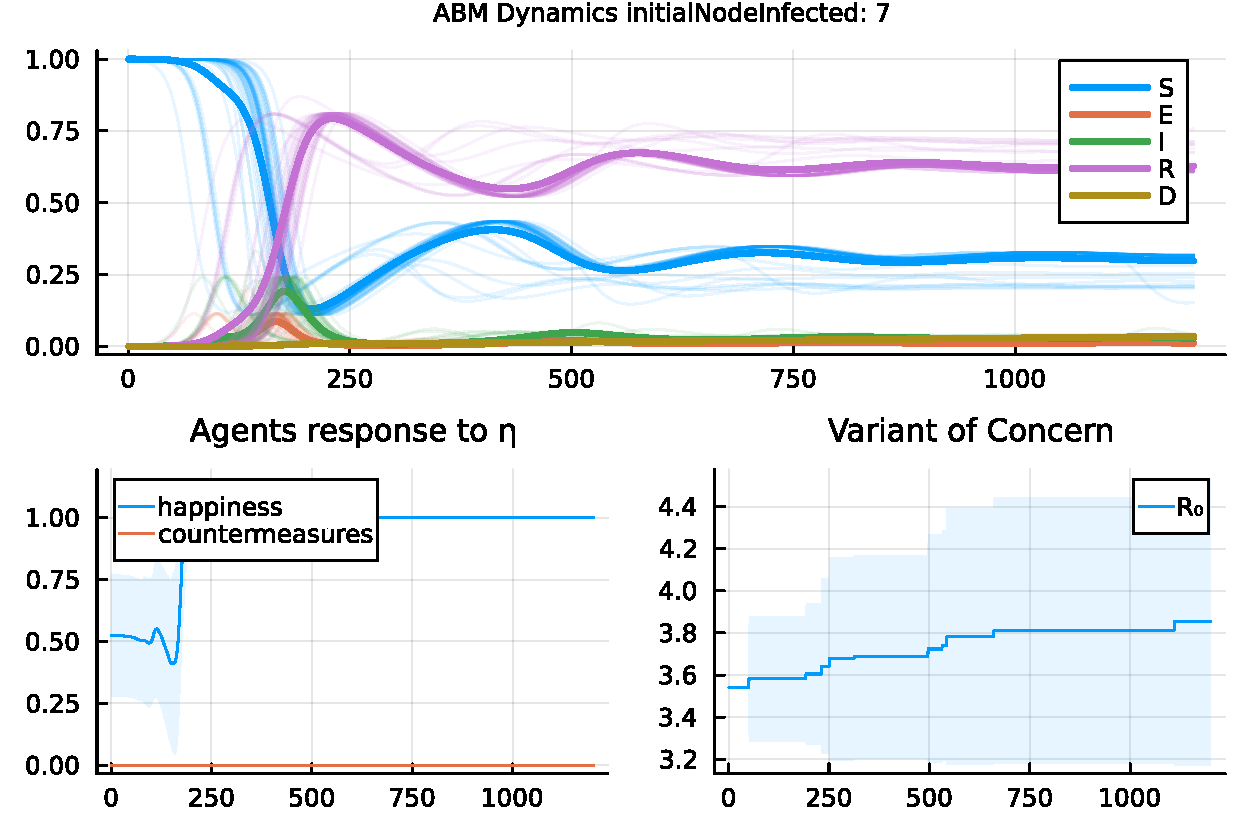
\includegraphics[width=\textwidth]{img/SocialNetworkABM_3_II.pdf}
		\caption{Grafico per la comparazione sul numero di nodi infetti di partenza. Numero nodi infetti iniziali 7}
		\label{fig:comparison_init_node_inf_7}
	\end{subfigure}
	\hfill
	\begin{subfigure}[b]{0.45\textwidth}
		\centering
		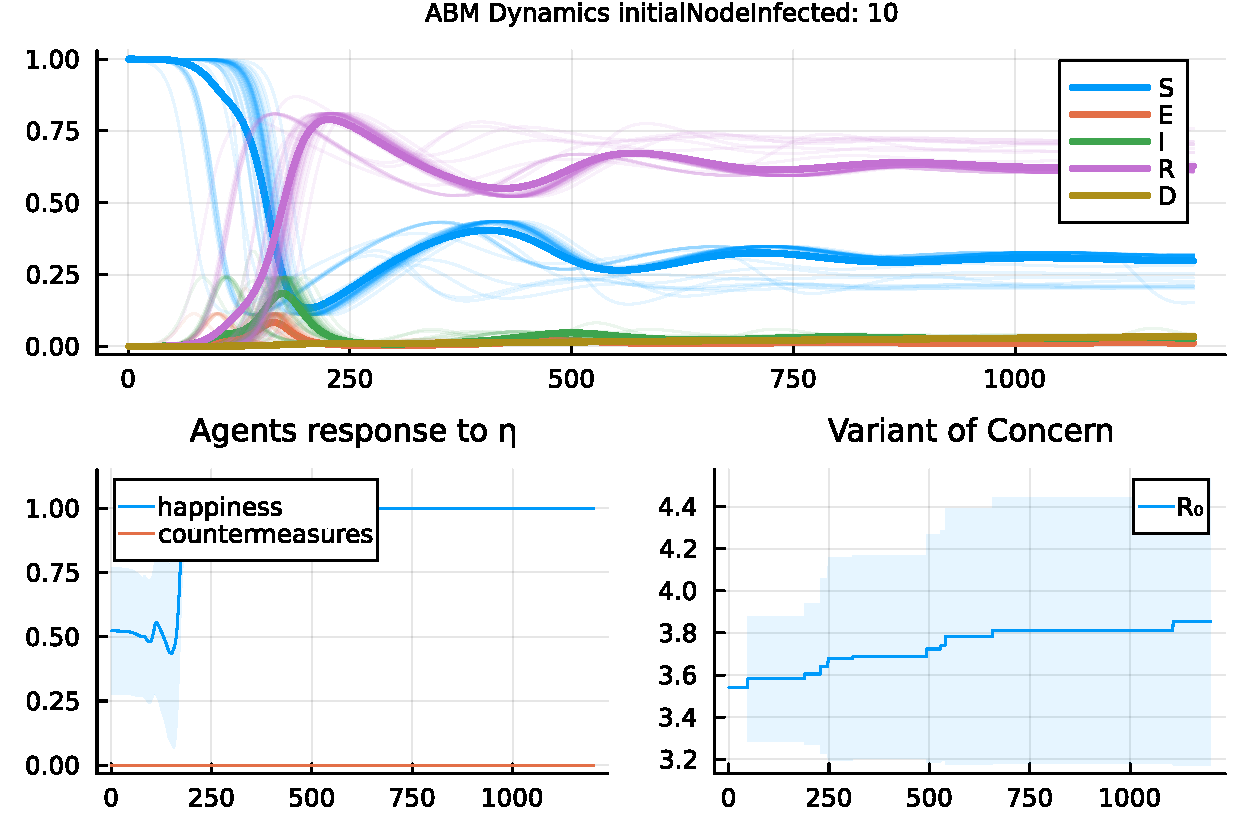
\includegraphics[width=\textwidth]{img/SocialNetworkABM_4_II.pdf}
		\caption{Grafico per la comparazione sul numero di nodi infetti di partenza. Numero nodi infetti iniziali 10}
		\label{fig:comparison_init_node_inf_10}
	\end{subfigure}
\end{figure}
\newpage

\subsection{Analisi del Comportamento in Base al Tasso di Migrazione}

L'analisi ha esaminato come il tasso di migrazione influenzi il 
comportamento del modello. Si è notato che un tasso di migrazione 
più alto ha portato a un picco di infetti più alto in un periodo 
di tempo più breve. Questo risultato è coerente con l'effetto 
della mobilità sulla diffusione delle malattie infettive.

\begin{figure}[!hb]
	\centering
	\begin{subfigure}[b]{0.45\textwidth}
		\centering
		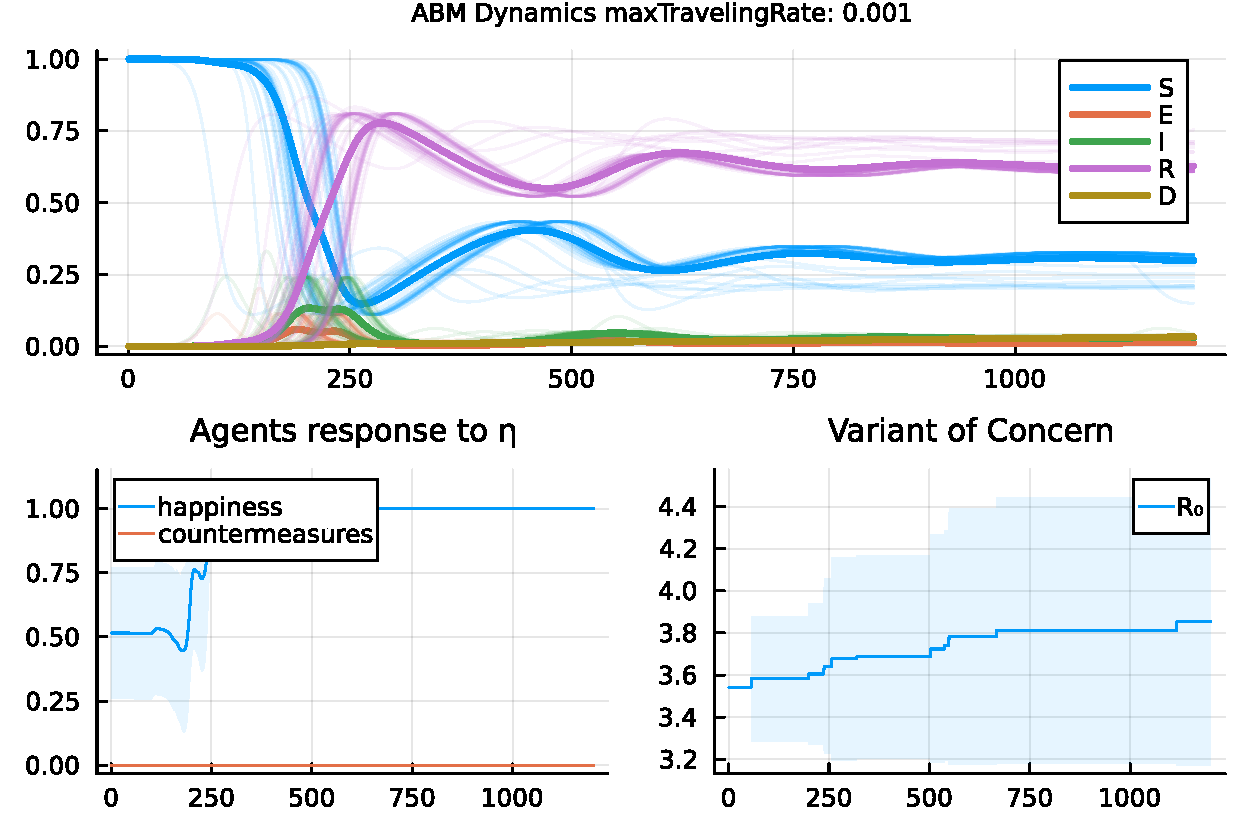
\includegraphics[width=\textwidth]{img/SocialNetworkABM_1_MTR.pdf}
		\caption{Grafico per la comparazione sul valore di migrazione. Valore di 0.001}
		\label{fig:comparison_maxTravelingRate_low}
	\end{subfigure}
	\hfill
	\begin{subfigure}[b]{0.45\textwidth}
		\centering
		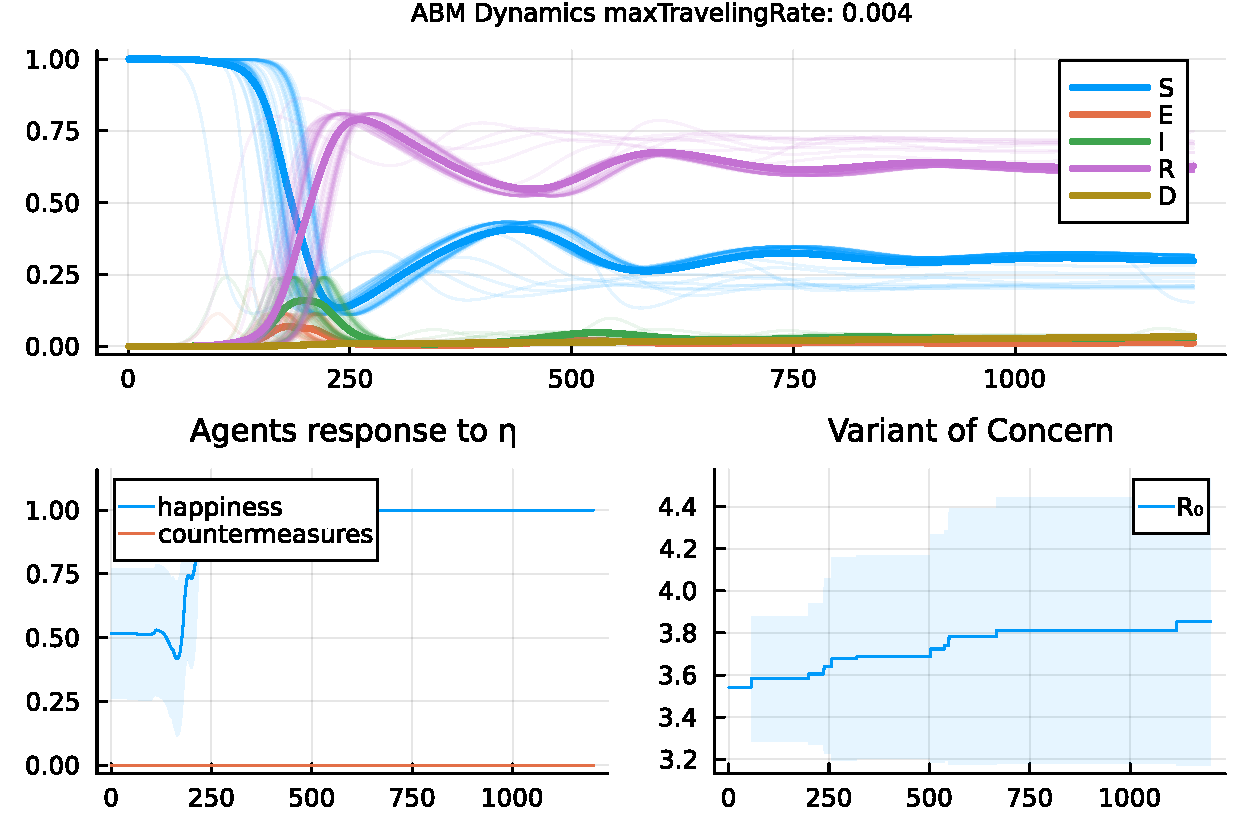
\includegraphics[width=\textwidth]{img/SocialNetworkABM_2_MTR.pdf}
		\caption{Grafico per la comparazione sul valore di migrazione. Valore di 0.004}
		\label{fig:comparison_maxTravelingRate_midl}
	\end{subfigure}
	\hfill
	\begin{subfigure}[b]{0.45\textwidth}
		\centering
		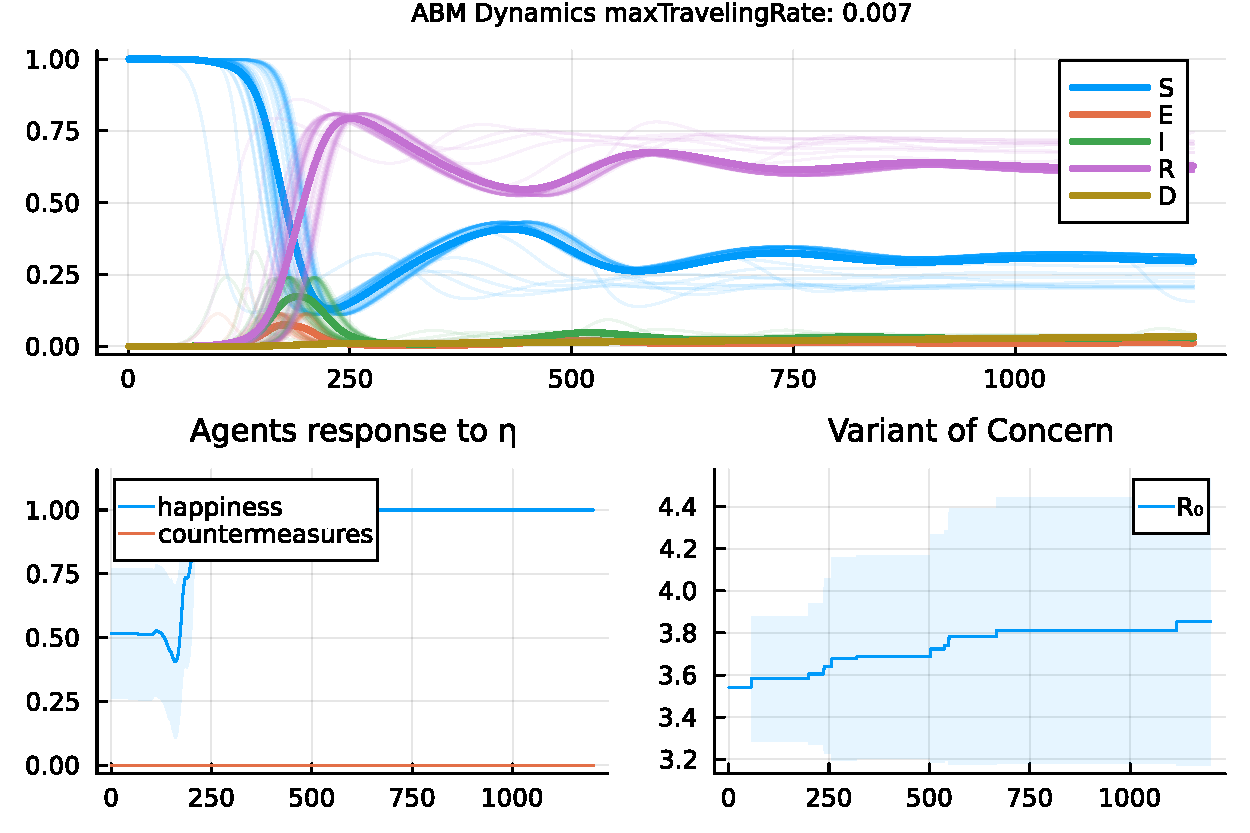
\includegraphics[width=\textwidth]{img/SocialNetworkABM_3_MTR.pdf}
		\caption{Grafico per la comparazione sul valore di migrazione. Valore di 0.007}
		\label{fig:comparison_maxTravelingRate_midh}
	\end{subfigure}
	\hfill
	\begin{subfigure}[b]{0.45\textwidth}
		\centering
		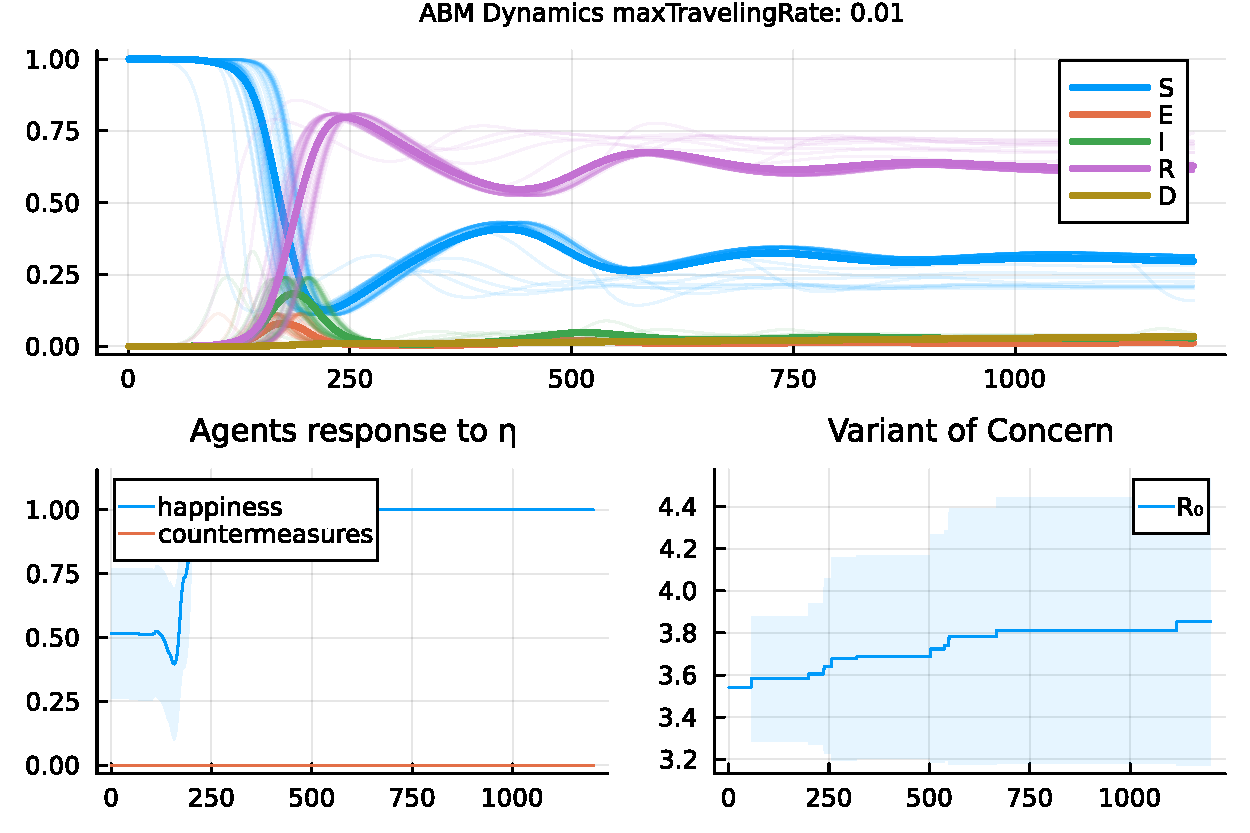
\includegraphics[width=\textwidth]{img/SocialNetworkABM_4_MTR.pdf}
		\caption{Grafico per la comparazione sul valore di migrazione. Valore di 0.01}
		\label{fig:comparison_maxTravelingRate_high}
	\end{subfigure}
\end{figure}
\newpage

\subsection{Analisi del Comportamento in Base al Numero di Nodi della Rete}

L'analisi ha esaminato come il numero di nodi della rete influenzi 
il comportamento del modello. Si è osservato che un numero maggiore
 di nodi ha portato a una diffusione più lenta e a picchi meno 
 ripidi ma più prolungati nel tempo. Questo risultato è influenzato 
 dalla topologia delle connessioni e dalla posizione del focolaio iniziale.

\begin{figure}[!hb]
	\centering
	\begin{subfigure}[b]{0.45\textwidth}
		\centering
		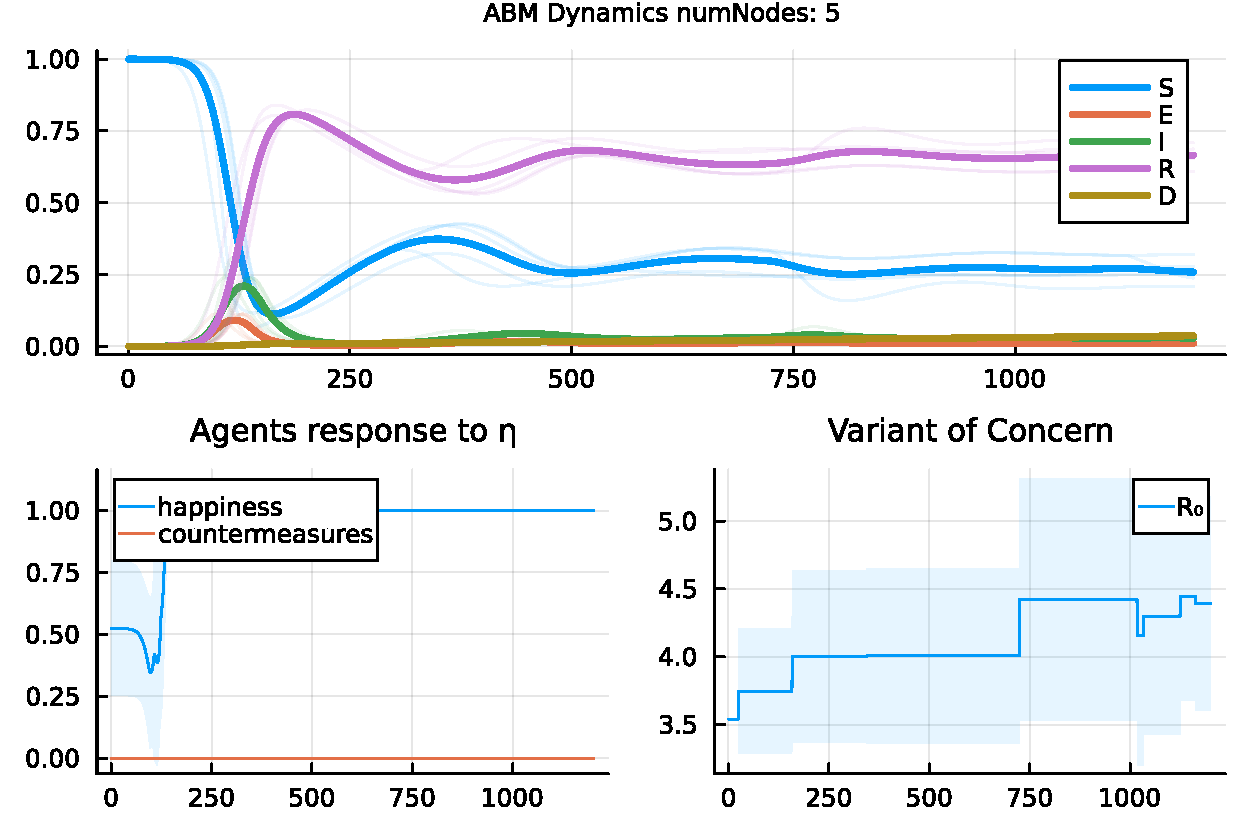
\includegraphics[width=\textwidth]{img/SocialNetworkABM_1_NN.pdf}
		\caption{Grafico per la comparazione sul numero di nodi della rete. Numero nodi 5}
		\label{fig:comparison_numberOfNodes_5}
	\end{subfigure}
	\hfill
	\begin{subfigure}[b]{0.45\textwidth}
		\centering
		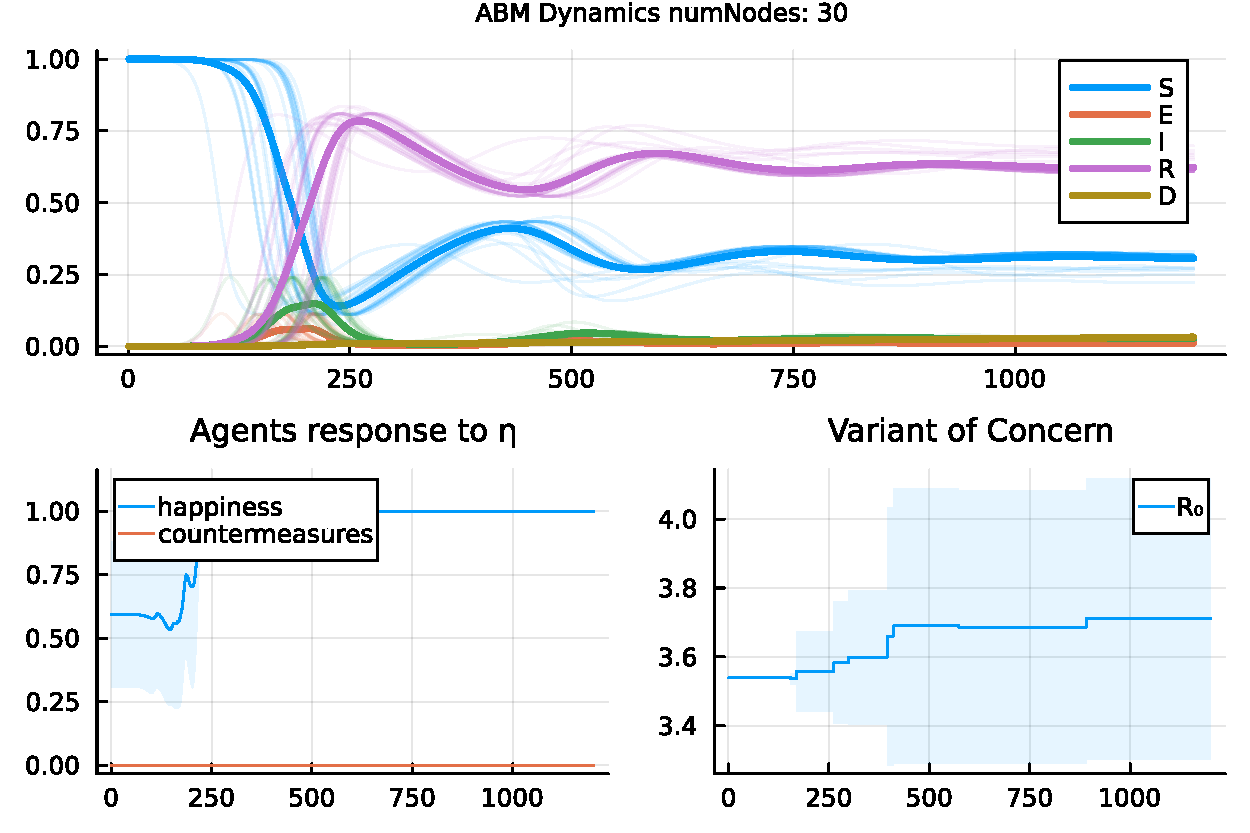
\includegraphics[width=\textwidth]{img/SocialNetworkABM_2_NN.pdf}
		\caption{Grafico per la comparazione sul numero di nodi della rete. Numero nodi 30}
		\label{fig:comparison_numberOfNodes_30}
	\end{subfigure}
	\hfill
	\begin{subfigure}[b]{0.45\textwidth}
		\centering
		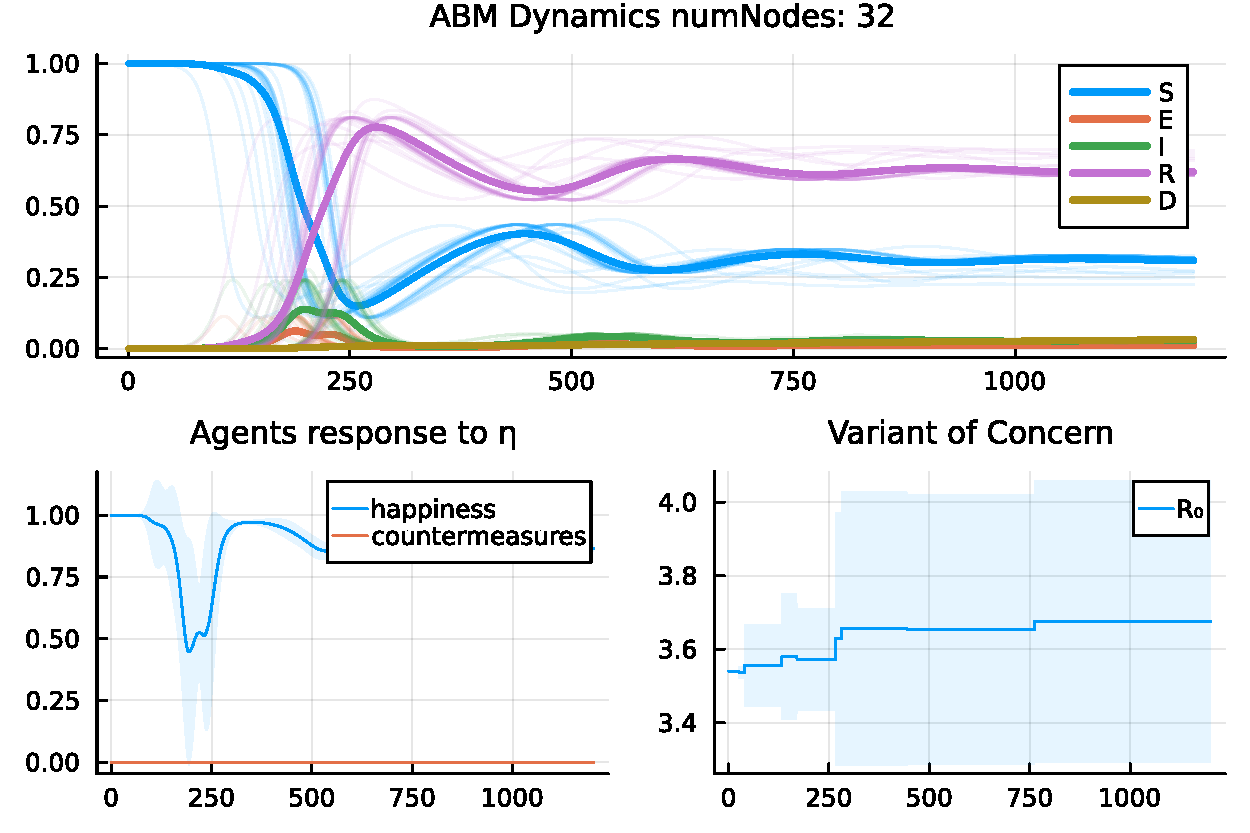
\includegraphics[width=\textwidth]{img/SocialNetworkABM_3_NN.pdf}
		\caption{Grafico per la comparazione sul numero di nodi della rete. Numero nodi 55}
		\label{fig:comparison_numberOfNodes_55}
	\end{subfigure}
	\hfill
	\begin{subfigure}[b]{0.45\textwidth}
		\centering
		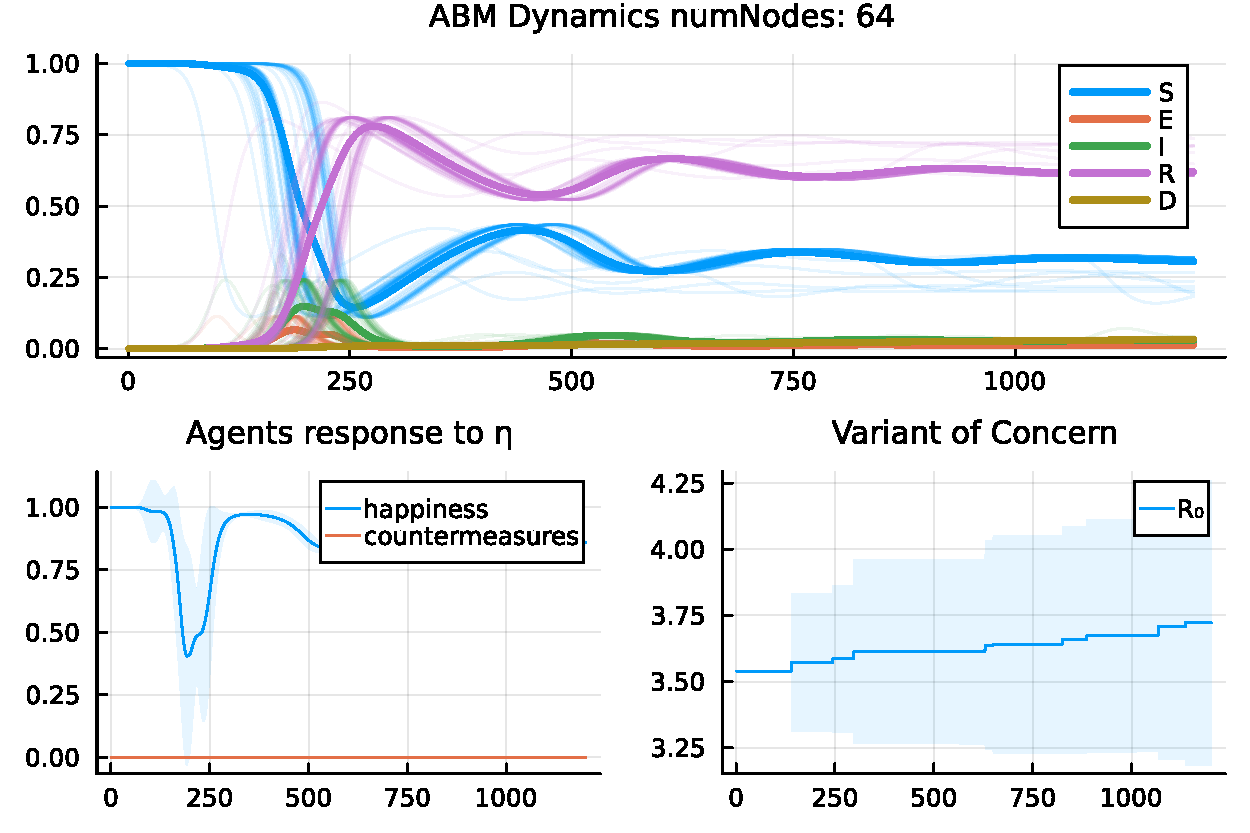
\includegraphics[width=\textwidth]{img/SocialNetworkABM_4_NN.pdf}
		\caption{Grafico per la comparazione sul numero di nodi della rete. Numero nodi 80}
		\label{fig:comparison_numberOfNodes_80}
	\end{subfigure}
\end{figure}
\newpage

\subsection{Analisi del Comportamento in Base alla Copertura della Rete}

L'analisi ha esaminato come la copertura della rete, rappresentata 
dal numero di archi, influenzi il comportamento del modello. 
Si è notato che una copertura bassa ha comportato un rallentamento 
della diffusione del virus, simile all'effetto di un lockdown. 
Questo risultato è coerente con l'importanza della mobilità nella 
diffusione delle malattie infettive e con il ruolo delle misure di 
contenimento.

\begin{figure}[!hb]
	\centering
	\begin{subfigure}[b]{0.3\textwidth}
		\centering
		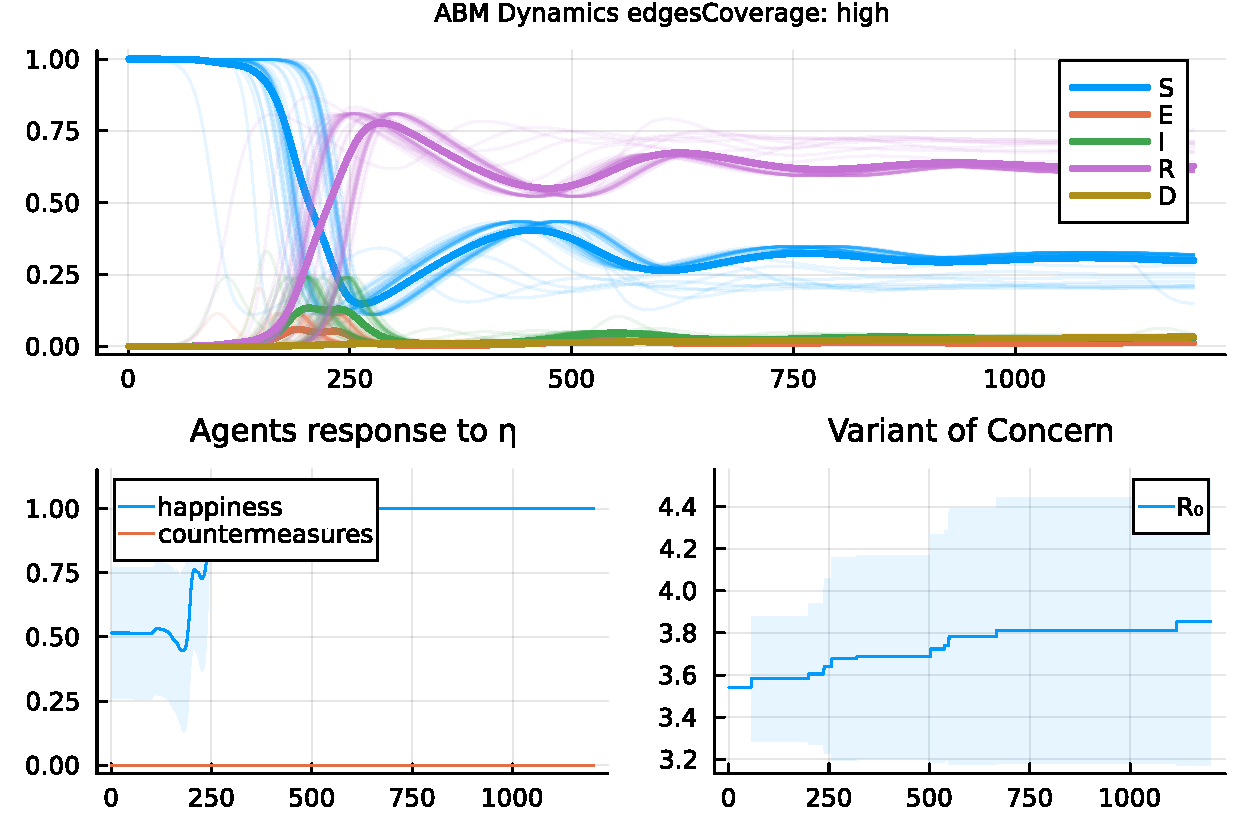
\includegraphics[width=\textwidth]{img/SocialNetworkABM_1_EC.pdf}
		\caption{Grafico per la comparazione sulla copertura della rete. Copertura alta}
		\label{fig:comparison_highCoverage}
	\end{subfigure}
	\hfill
	\begin{subfigure}[b]{0.3\textwidth}
		\centering
		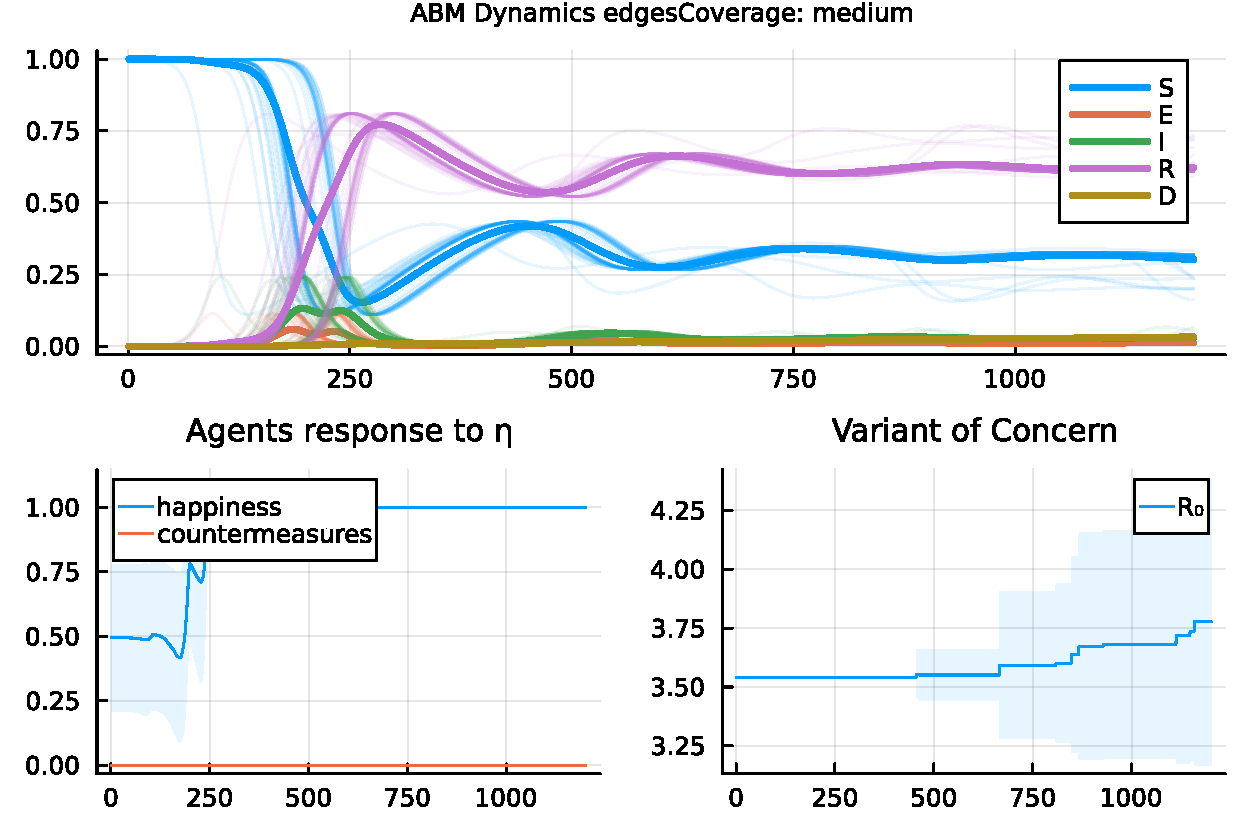
\includegraphics[width=\textwidth]{img/SocialNetworkABM_2_EC.pdf}
		\caption{Grafico per la comparazione sulla copertura della rete. Copertura media}
		\label{fig:comparison_mediumCoverage}
	\end{subfigure}
	\hfill
	\begin{subfigure}[b]{0.3\textwidth}
		\centering
		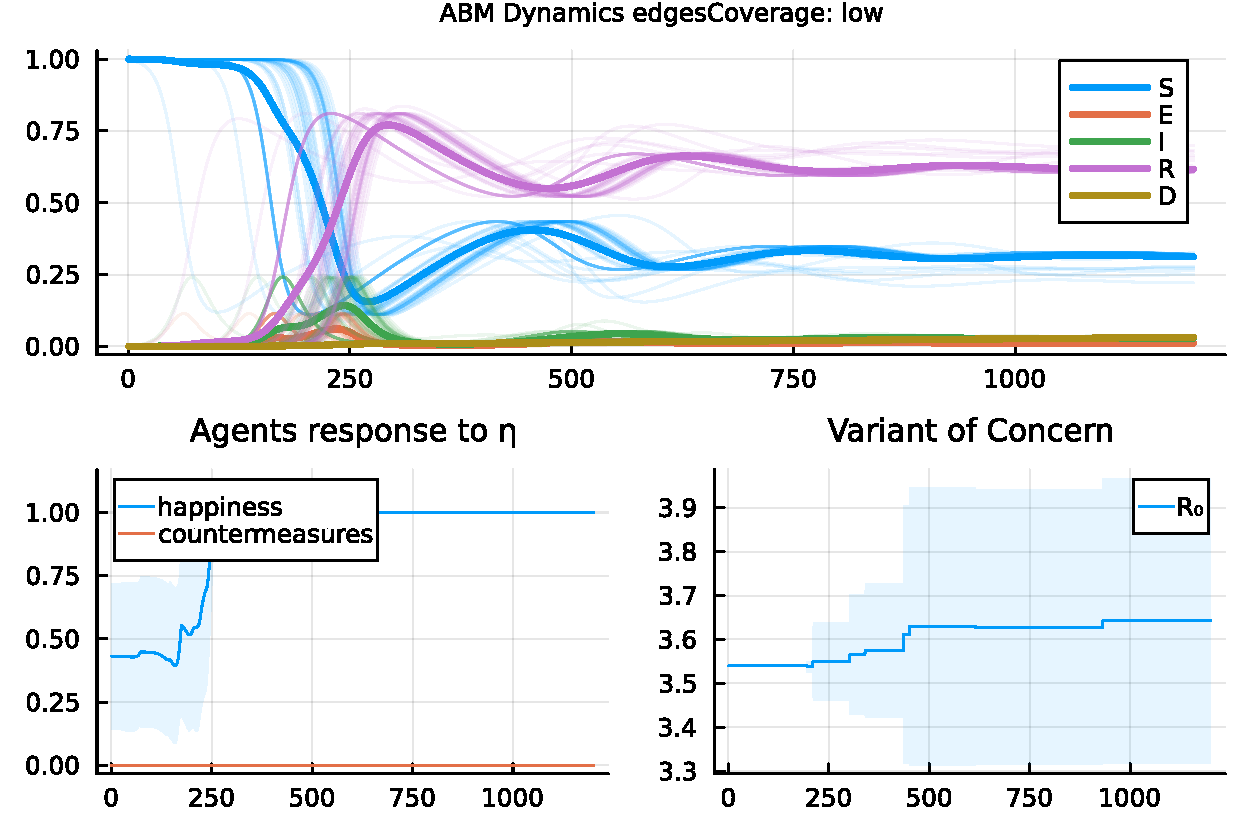
\includegraphics[width=\textwidth]{img/SocialNetworkABM_3_EC.pdf}
		\caption{Grafico per la comparazione sulla copertura della rete. Copertura bassa}
		\label{fig:comparison_lowCoverage}
	\end{subfigure}
\end{figure}

Inoltre, è stato osservato che il numero di varianti del virus 
(VOC) tende ad aumentare con il numero di nodi nella rete, 
suggerendo che più individui possono portare a un aumento delle 
mutazioni, ma la presenza di una bassa copertura può limitare la 
loro diffusione.

In sintesi, l'analisi ha evidenziato come vari parametri e 
condizioni possano influenzare il comportamento del modello 
epidemiologico, fornendo importanti informazioni per la 
comprensione e la gestione delle epidemie.